\documentclass[tikz,border=15pt]{standalone}
\usepackage{amsmath,amssymb}
\usetikzlibrary{calc}

\begin{document}
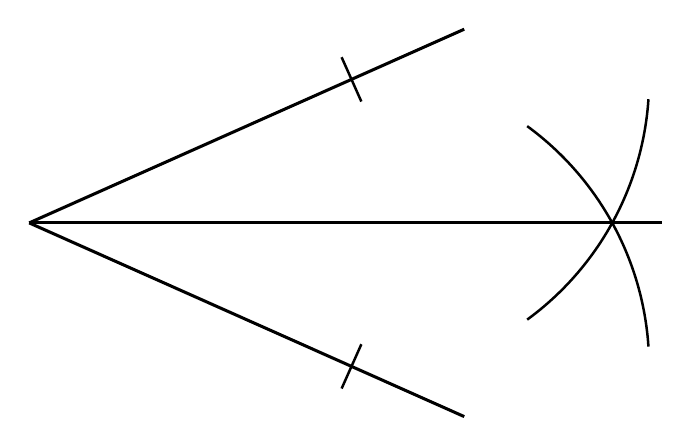
\begin{tikzpicture}[scale=1.4]
    \def\ang{24}
    \def\rarm{3.2}
    \def\rarc{2.7}
    
    \coordinate (V) at (0, 0);
    \coordinate (A) at ({\rarm*cos(\ang)}, {\rarm*sin(\ang)});
    \coordinate (B) at ({\rarm*cos(-\ang)}, {\rarm*sin(-\ang)});
    
    % The two arms of the original angle
    \draw[line width=1.1pt] (V) -- ({\rarm*1.35*cos(\ang)}, {\rarm*1.35*sin(\ang)});
    \draw[line width=1.1pt] (V) -- ({\rarm*1.35*cos(-\ang)}, {\rarm*1.35*sin(-\ang)});
    
    % Tick marks on the arms at distance rarm from vertex
    \draw[line width=0.9pt] ($(A) + ({\ang+90}:0.22)$) -- ($(A) + ({\ang-90}:0.22)$);
    \draw[line width=0.9pt] ($(B) + ({-\ang+90}:0.22)$) -- ($(B) + ({-\ang-90}:0.22)$);
    
    % Intersecting compass arcs from A and B
    % Center A, radius rarc
    % Arc from A crosses y=0 at x = rarm*cos(ang) + sqrt(rarc^2 - (rarm*sin(ang))^2)
    % Angle from A to intersection point is -asin((rarm*sin(ang))/rarc)
    \pgfmathsetmacro{\midangA}{-asin((\rarm*sin(\ang))/\rarc)}
    \pgfmathsetmacro{\midangB}{asin((\rarm*sin(\ang))/\rarc)}
    
    \draw[line width=0.9pt] ($(A) + ({\midangA - 25}:\rarc)$) arc ({\midangA - 25}:{\midangA + 25}:\rarc);
    \draw[line width=0.9pt] ($(B) + ({\midangB - 25}:\rarc)$) arc ({\midangB - 25}:{\midangB + 25}:\rarc);
    
    % Bisector line passing through vertex and the arc intersection
    \pgfmathsetmacro{\xP}{{\rarm*cos(\ang) + sqrt(\rarc*\rarc - (\rarm*sin(\ang))*(\rarm*sin(\ang)))}}
    \draw[line width=1.1pt] (V) -- ({\xP + 0.45}, 0);
    
\end{tikzpicture}
\end{document}
